\section{Изучение поставленной задачи с помощью\\компьютерного моделирования}

\subsection{Математическая постановка исходной задачи}

Запишем \textbf{общее уравнение непрерывности} в дифференциальной форме:

\begin{equation}\label{eq:main}
\rho_t(\bar{x},t) + div \bar{J}(\bar{x},t) = f(\bar{x},t)
\end{equation}

Оно представляет собой сильную (локальную) форму закона сохранения и выражает связь между потоком $\bar{J} (\bar{x},t)$ и концетрацией (температурой) $\rho(\bar{x},t)$.

Чтобы корректно поставить задачу решения \ref{eq:main} необходимо дополнить его ещё одним условием \--- в данной работе оно представлено \textbf{законом диффузии с конвекцией} с отклоняющимся аргументом:

\begin{equation}\label{eq:diffusion-convection}
\bar{J}(\bar{x},t+\tau) = -a^2 \nabla \rho(\bar{x},t) + \bar{V}(\bar{x},t) \rho(\bar{x},t)
\end{equation}

В дальнейшем уравнение \ref{eq:main} будет классифицировано с точки зрения теории дифференциальных уравнений с отклоняющимся аргументом. Предварительно приведем необходимую для исследования информацию.

\subsection{Теория дифференциальных уравнений\\с отклоняющимся аргументом}

\subsubsection{Базовые понятия и определения}

\textbf{Дифференциальными уравнениями с отклоняющимся аргументом} называются дифференциальные уравнения, в которые неизвестная функция и её проиводные входят, вообще говоря, при различных значениях аргумента.

Хотя уравнения с отклоняющимся аргументом по виду очень похожи на обыкновенные дифференциальные уравнения, факт отклонения аргумента усложняет их анализ.

Рассмотрим простейший пример

\begin{equation}\label{eq:example}
\dot{x}(t) = f(t,x(t),x(t-\tau)),
\end{equation}

где $\tau$ \--- положительная константа.

Для начала отметим, что для решения задачи Коши уже недостаточно задать одно начальное условие $x(t_0)=x_0$, ведь необходимо знать исходные значения на всем отрезке $[t_0-\tau,t_0]$, т.е задать функцию $x(t)$, определенную на отрезке $[t_0-\tau,t_0]$ \--- \textbf{начальную функцию} (в зарубежной литературе \textbf{history function} или \textbf{initial function}).

\subsubsection{Простейшая модель с запаздыванием}

Для примера рассмотрим две задачи Коши: одну для обыкновенного дифференциального уравнения, другую \--- для уравнения с отклонением по аргументу:

\begin{equation}\label{eq:no-delay}
\left\{
\begin{aligned}
x'(t) = x(t), \quad t>0\\
x(0) = 1
\end{aligned}
\right.
\end{equation}

\begin{equation}\label{eq:delay}
\left\{
\begin{aligned}
y'(t) = y(t-1), \quad t>0\\
y(t) = 1, \quad -1 \leq t \leq 0
\end{aligned}
\right.
\end{equation}

Методы решения подобных уравнений с запаздыванием будут рассмотрены в работе позже, а пока построим графики этих решений:

\begin{center}
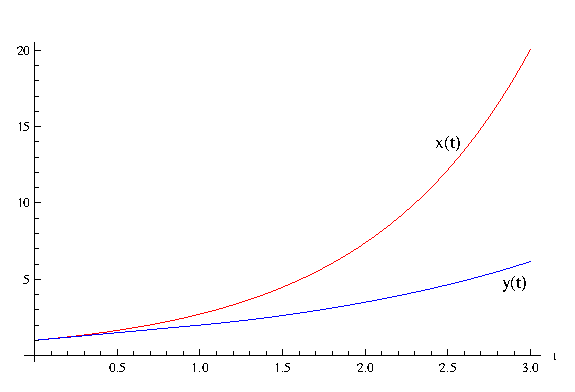
\includegraphics[width=0.65\textwidth]{./1_modelling/comparison.eps}
\end{center}

Наглядно видно, что решения различны. Позже будет приведено аналитическое решение задачи \ref{eq:delay} и доказано, что $y(t)$ всегда возрастает медленнее экспоненциального решения, т.е. $x(t)$.

Также решение зависит от начальной функции: для примера рассмотрим такую задачу:

\begin{equation}\label{eq:no-delay-history}
\left\{
\begin{aligned}
y'_h(t) = y_h(t-1), \quad t>0\\
y_h(t) = 1+t, \quad -1 \leq t \leq 0
\end{aligned}
\right.
\end{equation}

Отметим, что $y_h(0) = y(0) = 1$.

Построим решения на одном графике: